\documentclass[]{article}
\usepackage{lmodern}
\usepackage{amssymb,amsmath}
\usepackage{ifxetex,ifluatex}
\usepackage{fixltx2e} % provides \textsubscript
\ifnum 0\ifxetex 1\fi\ifluatex 1\fi=0 % if pdftex
  \usepackage[T1]{fontenc}
  \usepackage[utf8]{inputenc}
\else % if luatex or xelatex
  \ifxetex
    \usepackage{mathspec}
  \else
    \usepackage{fontspec}
  \fi
  \defaultfontfeatures{Ligatures=TeX,Scale=MatchLowercase}
\fi
% use upquote if available, for straight quotes in verbatim environments
\IfFileExists{upquote.sty}{\usepackage{upquote}}{}
% use microtype if available
\IfFileExists{microtype.sty}{%
\usepackage{microtype}
\UseMicrotypeSet[protrusion]{basicmath} % disable protrusion for tt fonts
}{}
\usepackage[margin=1in]{geometry}
\usepackage{hyperref}
\hypersetup{unicode=true,
            pdftitle={Homework 1},
            pdfauthor={Noah Kawasaki},
            pdfborder={0 0 0},
            breaklinks=true}
\urlstyle{same}  % don't use monospace font for urls
\usepackage{color}
\usepackage{fancyvrb}
\newcommand{\VerbBar}{|}
\newcommand{\VERB}{\Verb[commandchars=\\\{\}]}
\DefineVerbatimEnvironment{Highlighting}{Verbatim}{commandchars=\\\{\}}
% Add ',fontsize=\small' for more characters per line
\usepackage{framed}
\definecolor{shadecolor}{RGB}{248,248,248}
\newenvironment{Shaded}{\begin{snugshade}}{\end{snugshade}}
\newcommand{\KeywordTok}[1]{\textcolor[rgb]{0.13,0.29,0.53}{\textbf{#1}}}
\newcommand{\DataTypeTok}[1]{\textcolor[rgb]{0.13,0.29,0.53}{#1}}
\newcommand{\DecValTok}[1]{\textcolor[rgb]{0.00,0.00,0.81}{#1}}
\newcommand{\BaseNTok}[1]{\textcolor[rgb]{0.00,0.00,0.81}{#1}}
\newcommand{\FloatTok}[1]{\textcolor[rgb]{0.00,0.00,0.81}{#1}}
\newcommand{\ConstantTok}[1]{\textcolor[rgb]{0.00,0.00,0.00}{#1}}
\newcommand{\CharTok}[1]{\textcolor[rgb]{0.31,0.60,0.02}{#1}}
\newcommand{\SpecialCharTok}[1]{\textcolor[rgb]{0.00,0.00,0.00}{#1}}
\newcommand{\StringTok}[1]{\textcolor[rgb]{0.31,0.60,0.02}{#1}}
\newcommand{\VerbatimStringTok}[1]{\textcolor[rgb]{0.31,0.60,0.02}{#1}}
\newcommand{\SpecialStringTok}[1]{\textcolor[rgb]{0.31,0.60,0.02}{#1}}
\newcommand{\ImportTok}[1]{#1}
\newcommand{\CommentTok}[1]{\textcolor[rgb]{0.56,0.35,0.01}{\textit{#1}}}
\newcommand{\DocumentationTok}[1]{\textcolor[rgb]{0.56,0.35,0.01}{\textbf{\textit{#1}}}}
\newcommand{\AnnotationTok}[1]{\textcolor[rgb]{0.56,0.35,0.01}{\textbf{\textit{#1}}}}
\newcommand{\CommentVarTok}[1]{\textcolor[rgb]{0.56,0.35,0.01}{\textbf{\textit{#1}}}}
\newcommand{\OtherTok}[1]{\textcolor[rgb]{0.56,0.35,0.01}{#1}}
\newcommand{\FunctionTok}[1]{\textcolor[rgb]{0.00,0.00,0.00}{#1}}
\newcommand{\VariableTok}[1]{\textcolor[rgb]{0.00,0.00,0.00}{#1}}
\newcommand{\ControlFlowTok}[1]{\textcolor[rgb]{0.13,0.29,0.53}{\textbf{#1}}}
\newcommand{\OperatorTok}[1]{\textcolor[rgb]{0.81,0.36,0.00}{\textbf{#1}}}
\newcommand{\BuiltInTok}[1]{#1}
\newcommand{\ExtensionTok}[1]{#1}
\newcommand{\PreprocessorTok}[1]{\textcolor[rgb]{0.56,0.35,0.01}{\textit{#1}}}
\newcommand{\AttributeTok}[1]{\textcolor[rgb]{0.77,0.63,0.00}{#1}}
\newcommand{\RegionMarkerTok}[1]{#1}
\newcommand{\InformationTok}[1]{\textcolor[rgb]{0.56,0.35,0.01}{\textbf{\textit{#1}}}}
\newcommand{\WarningTok}[1]{\textcolor[rgb]{0.56,0.35,0.01}{\textbf{\textit{#1}}}}
\newcommand{\AlertTok}[1]{\textcolor[rgb]{0.94,0.16,0.16}{#1}}
\newcommand{\ErrorTok}[1]{\textcolor[rgb]{0.64,0.00,0.00}{\textbf{#1}}}
\newcommand{\NormalTok}[1]{#1}
\usepackage{graphicx,grffile}
\makeatletter
\def\maxwidth{\ifdim\Gin@nat@width>\linewidth\linewidth\else\Gin@nat@width\fi}
\def\maxheight{\ifdim\Gin@nat@height>\textheight\textheight\else\Gin@nat@height\fi}
\makeatother
% Scale images if necessary, so that they will not overflow the page
% margins by default, and it is still possible to overwrite the defaults
% using explicit options in \includegraphics[width, height, ...]{}
\setkeys{Gin}{width=\maxwidth,height=\maxheight,keepaspectratio}
\IfFileExists{parskip.sty}{%
\usepackage{parskip}
}{% else
\setlength{\parindent}{0pt}
\setlength{\parskip}{6pt plus 2pt minus 1pt}
}
\setlength{\emergencystretch}{3em}  % prevent overfull lines
\providecommand{\tightlist}{%
  \setlength{\itemsep}{0pt}\setlength{\parskip}{0pt}}
\setcounter{secnumdepth}{0}
% Redefines (sub)paragraphs to behave more like sections
\ifx\paragraph\undefined\else
\let\oldparagraph\paragraph
\renewcommand{\paragraph}[1]{\oldparagraph{#1}\mbox{}}
\fi
\ifx\subparagraph\undefined\else
\let\oldsubparagraph\subparagraph
\renewcommand{\subparagraph}[1]{\oldsubparagraph{#1}\mbox{}}
\fi

%%% Use protect on footnotes to avoid problems with footnotes in titles
\let\rmarkdownfootnote\footnote%
\def\footnote{\protect\rmarkdownfootnote}

%%% Change title format to be more compact
\usepackage{titling}

% Create subtitle command for use in maketitle
\newcommand{\subtitle}[1]{
  \posttitle{
    \begin{center}\large#1\end{center}
    }
}

\setlength{\droptitle}{-2em}
  \title{Homework 1}
  \pretitle{\vspace{\droptitle}\centering\huge}
  \posttitle{\par}
  \author{Noah Kawasaki}
  \preauthor{\centering\large\emph}
  \postauthor{\par}
  \predate{\centering\large\emph}
  \postdate{\par}
  \date{4-13-2017}


\begin{document}
\maketitle

\subsection{Part 1: Review Questions}\label{part-1-review-questions}

Consider the following (actual) monthly adjusted closing price data for
Starbucks stock over the period December 2011 through December 2012:

\paragraph{Create dataframe}\label{create-dataframe}

\begin{Shaded}
\begin{Highlighting}[]
\CommentTok{# Vectors}
\NormalTok{date <-}\StringTok{ }\KeywordTok{c}\NormalTok{(}\StringTok{'12/31/2011'}\NormalTok{, }\StringTok{'1/31/2012'}\NormalTok{, }\StringTok{'2/28/2012'}\NormalTok{, }\StringTok{'3/31/2012'}\NormalTok{, }\StringTok{'4/30/2012'}\NormalTok{, }\StringTok{'5/31/2012'}\NormalTok{, }\StringTok{'6/30/2012'}\NormalTok{, }\StringTok{'7/31/2012'}\NormalTok{, }\StringTok{'8/31/2012'}\NormalTok{, }\StringTok{'9/30/2012'}\NormalTok{, }\StringTok{'10/31/2012'}\NormalTok{, }\StringTok{'11/30/2012'}\NormalTok{, }\StringTok{'12/31/2012'}\NormalTok{)}
\NormalTok{price <-}\StringTok{ }\KeywordTok{c}\NormalTok{(}\FloatTok{44.89}\NormalTok{, }\FloatTok{46.76}\NormalTok{, }\FloatTok{47.55}\NormalTok{, }\FloatTok{54.73}\NormalTok{, }\FloatTok{56.17}\NormalTok{, }\FloatTok{53.91}\NormalTok{, }\FloatTok{52.37}\NormalTok{, }\FloatTok{44.47}\NormalTok{, }\FloatTok{48.91}\NormalTok{, }\FloatTok{50.00}\NormalTok{, }\FloatTok{45.26}\NormalTok{, }\FloatTok{51.36}\NormalTok{, }\FloatTok{53.10}\NormalTok{)}

\NormalTok{df <-}\StringTok{ }\KeywordTok{data.frame}\NormalTok{(date, price)}
\CommentTok{# Reformat as date type}
\NormalTok{df}\OperatorTok{$}\NormalTok{date <-}\StringTok{ }\KeywordTok{as.Date}\NormalTok{(df}\OperatorTok{$}\NormalTok{date, }\DataTypeTok{format=}\StringTok{"%m/%d/%Y"}\NormalTok{)}

\NormalTok{df}
\end{Highlighting}
\end{Shaded}

\begin{verbatim}
##          date price
## 1  2011-12-31 44.89
## 2  2012-01-31 46.76
## 3  2012-02-28 47.55
## 4  2012-03-31 54.73
## 5  2012-04-30 56.17
## 6  2012-05-31 53.91
## 7  2012-06-30 52.37
## 8  2012-07-31 44.47
## 9  2012-08-31 48.91
## 10 2012-09-30 50.00
## 11 2012-10-31 45.26
## 12 2012-11-30 51.36
## 13 2012-12-31 53.10
\end{verbatim}

\paragraph{\texorpdfstring{1. Using the data in the table, what is the
\emph{simple monthly return} between the end of December, 2011 and the
end of January 2012? If you invested \$10,000 in Starbucks at the end of
December 2011, how much would the investment be worth at the end of
January
2012?}{1. Using the data in the table, what is the simple monthly return between the end of December, 2011 and the end of January 2012? If you invested \$10,000 in Starbucks at the end of December 2011, how much would the investment be worth at the end of January 2012?}}\label{using-the-data-in-the-table-what-is-the-simple-monthly-return-between-the-end-of-december-2011-and-the-end-of-january-2012-if-you-invested-10000-in-starbucks-at-the-end-of-december-2011-how-much-would-the-investment-be-worth-at-the-end-of-january-2012}

\[R_t = \frac{P_t - P_{t-1}}{P_{t-1}}\]

\begin{Shaded}
\begin{Highlighting}[]
\NormalTok{Rt <-}\StringTok{ }\NormalTok{(}\FloatTok{46.76}\OperatorTok{-}\FloatTok{44.89}\NormalTok{)}\OperatorTok{/}\FloatTok{44.89}
\NormalTok{Rt}
\end{Highlighting}
\end{Shaded}

\begin{verbatim}
## [1] 0.04165738
\end{verbatim}

\[ FV = 10000(1+R_t)\]

\begin{Shaded}
\begin{Highlighting}[]
\NormalTok{FV <-}\StringTok{ }\DecValTok{10000}\OperatorTok{*}\NormalTok{(}\DecValTok{1}\OperatorTok{+}\NormalTok{Rt)}
\NormalTok{FV}
\end{Highlighting}
\end{Shaded}

\begin{verbatim}
## [1] 10416.57
\end{verbatim}

\paragraph{\texorpdfstring{2. Using the data in the table, what is the
\emph{continuously compounded monthly return} between December, 2011 and
January 2012? Convert this continuously compounded return to a simple
return (you should get the same answer as in part
1).}{2. Using the data in the table, what is the continuously compounded monthly return between December, 2011 and January 2012? Convert this continuously compounded return to a simple return (you should get the same answer as in part 1).}}\label{using-the-data-in-the-table-what-is-the-continuously-compounded-monthly-return-between-december-2011-and-january-2012-convert-this-continuously-compounded-return-to-a-simple-return-you-should-get-the-same-answer-as-in-part-1.}

\[r_t = ln(1+R_t) = ln\Big(\frac{P_t}{P_{t-1}}\Big)\]

\begin{Shaded}
\begin{Highlighting}[]
\NormalTok{rt <-}\StringTok{ }\KeywordTok{log}\NormalTok{((}\FloatTok{46.76}\OperatorTok{/}\FloatTok{44.89}\NormalTok{))}
\NormalTok{rt}
\end{Highlighting}
\end{Shaded}

\begin{verbatim}
## [1] 0.04081308
\end{verbatim}

\[R_t = e^{r_t} - 1\]

\begin{Shaded}
\begin{Highlighting}[]
\NormalTok{rt_converted <-}\StringTok{ }\KeywordTok{exp}\NormalTok{(rt) }\OperatorTok{-}\StringTok{ }\DecValTok{1}
\NormalTok{rt_converted}
\end{Highlighting}
\end{Shaded}

\begin{verbatim}
## [1] 0.04165738
\end{verbatim}

Note that this is the same answer from part 1.

\paragraph{\texorpdfstring{3. Assuming that the \emph{simple monthly
return} you computed in part 1 is the same for 12 months, what is the
\emph{simple annual return} with monthly
compounding?}{3. Assuming that the simple monthly return you computed in part 1 is the same for 12 months, what is the simple annual return with monthly compounding?}}\label{assuming-that-the-simple-monthly-return-you-computed-in-part-1-is-the-same-for-12-months-what-is-the-simple-annual-return-with-monthly-compounding}

\[R_t(12) = R_A = (1+R_t)^{12} - 1\]

\begin{Shaded}
\begin{Highlighting}[]
\NormalTok{Rt_}\DecValTok{12}\NormalTok{ <-}\StringTok{ }\NormalTok{(}\DecValTok{1} \OperatorTok{+}\StringTok{ }\NormalTok{Rt)}\OperatorTok{^}\DecValTok{12} \OperatorTok{-}\StringTok{ }\DecValTok{1}
\NormalTok{Rt_}\DecValTok{12}
\end{Highlighting}
\end{Shaded}

\begin{verbatim}
## [1] 0.6319196
\end{verbatim}

\paragraph{\texorpdfstring{4. Assuming that the \emph{continuously
compounded monthly return} you computed in part 2 is the same for 12
months, what is the \emph{continuously compounded annual
return}?}{4. Assuming that the continuously compounded monthly return you computed in part 2 is the same for 12 months, what is the continuously compounded annual return?}}\label{assuming-that-the-continuously-compounded-monthly-return-you-computed-in-part-2-is-the-same-for-12-months-what-is-the-continuously-compounded-annual-return}

\[r_t(12) = r_A = 12*r_t\]

\begin{Shaded}
\begin{Highlighting}[]
\NormalTok{ra <-}\StringTok{ }\DecValTok{12}\OperatorTok{*}\NormalTok{rt}
\NormalTok{ra}
\end{Highlighting}
\end{Shaded}

\begin{verbatim}
## [1] 0.489757
\end{verbatim}

\paragraph{\texorpdfstring{5. Using the data in the table, compute the
\emph{actual simple annual return} between December 2011 and December
2012. If you invested \$10,000 in Starbucks at the end of December 2011,
how much would the investment be worth at the end of December 2012?
Compare with your result in part
3.}{5. Using the data in the table, compute the actual simple annual return between December 2011 and December 2012. If you invested \$10,000 in Starbucks at the end of December 2011, how much would the investment be worth at the end of December 2012? Compare with your result in part 3.}}\label{using-the-data-in-the-table-compute-the-actual-simple-annual-return-between-december-2011-and-december-2012.-if-you-invested-10000-in-starbucks-at-the-end-of-december-2011-how-much-would-the-investment-be-worth-at-the-end-of-december-2012-compare-with-your-result-in-part-3.}

\[R_t(12) = R_A = \frac{P_t - P_{t-12}}{P_{t-12}} \]

\begin{Shaded}
\begin{Highlighting}[]
\NormalTok{RA <-}\StringTok{ }\NormalTok{(}\FloatTok{53.10}\OperatorTok{-}\FloatTok{44.89}\NormalTok{)}\OperatorTok{/}\FloatTok{44.89}
\NormalTok{RA}
\end{Highlighting}
\end{Shaded}

\begin{verbatim}
## [1] 0.1828915
\end{verbatim}

\[ FV = 10000(1+R_A)\]

\begin{Shaded}
\begin{Highlighting}[]
\NormalTok{FV_A <-}\StringTok{ }\DecValTok{10000}\OperatorTok{*}\NormalTok{(}\DecValTok{1}\OperatorTok{+}\NormalTok{RA) }
\NormalTok{FV_A}
\end{Highlighting}
\end{Shaded}

\begin{verbatim}
## [1] 11828.92
\end{verbatim}

\paragraph{6. Using the data in the table, compute the actual annual
continuously compounded return between December 2011 and December 2012.
Compare with your result in part (4). Convert this continuously
compounded return to a simple return (you should get the same answer as
in part
5).}\label{using-the-data-in-the-table-compute-the-actual-annual-continuously-compounded-return-between-december-2011-and-december-2012.-compare-with-your-result-in-part-4.-convert-this-continuously-compounded-return-to-a-simple-return-you-should-get-the-same-answer-as-in-part-5.}

\[r_A  = r_t(12) = ln(1+R_t(12)) = ln\Big(\frac{P_t}{P_{t-12}}\Big)\]

\begin{Shaded}
\begin{Highlighting}[]
\NormalTok{ra <-}\StringTok{ }\KeywordTok{log}\NormalTok{(}\FloatTok{53.10}\OperatorTok{/}\FloatTok{44.89}\NormalTok{)}
\NormalTok{ra}
\end{Highlighting}
\end{Shaded}

\begin{verbatim}
## [1] 0.1679619
\end{verbatim}

\[R_A = e^{r_A} - 1\]

\begin{Shaded}
\begin{Highlighting}[]
\NormalTok{RA_converted <-}\StringTok{ }\KeywordTok{exp}\NormalTok{(ra) }\OperatorTok{-}\StringTok{ }\DecValTok{1}
\NormalTok{RA_converted}
\end{Highlighting}
\end{Shaded}

\begin{verbatim}
## [1] 0.1828915
\end{verbatim}

Note that this is the same answer as part 5.

\subsection{Part 2: R Exercises}\label{part-2-r-exercises}

\paragraph{1) Manipulate data}\label{manipulate-data}

\begin{Shaded}
\begin{Highlighting}[]
\NormalTok{starbucks =}\StringTok{ }\KeywordTok{read.csv}\NormalTok{(}\StringTok{'/Users/noahkawasaki/Desktop/ECON 147/Homework 1/sbuxPrices.csv'}\NormalTok{)}
\CommentTok{# Reformat as date type}
\NormalTok{starbucks}\OperatorTok{$}\NormalTok{Date <-}\StringTok{ }\KeywordTok{as.Date}\NormalTok{(starbucks}\OperatorTok{$}\NormalTok{Date, }\DataTypeTok{format=}\StringTok{"%m/%d/%Y"}\NormalTok{)}
\CommentTok{# Rename}
\KeywordTok{colnames}\NormalTok{(starbucks) <-}\StringTok{ }\KeywordTok{c}\NormalTok{(}\StringTok{'date'}\NormalTok{, }\StringTok{'price'}\NormalTok{)}

\KeywordTok{head}\NormalTok{(starbucks)}
\end{Highlighting}
\end{Shaded}

\begin{verbatim}
##         date    price
## 1 1998-03-01 2.323093
## 2 1998-04-01 2.467284
## 3 1998-05-01 2.460876
## 4 1998-06-01 2.739647
## 5 1998-07-01 2.146858
## 6 1998-08-01 1.618154
\end{verbatim}

\paragraph{2) Plot}\label{plot}

\begin{Shaded}
\begin{Highlighting}[]
\KeywordTok{ggplot}\NormalTok{(}\DataTypeTok{data=}\NormalTok{starbucks, }\DataTypeTok{mapping=}\KeywordTok{aes}\NormalTok{(date, price)) }\OperatorTok{+}
\StringTok{  }\KeywordTok{geom_line}\NormalTok{(}\DataTypeTok{color=}\StringTok{'#3796db'}\NormalTok{, }\DataTypeTok{lwd=}\DecValTok{1}\NormalTok{) }\OperatorTok{+}
\StringTok{  }\KeywordTok{ggtitle}\NormalTok{(}\StringTok{'Starbucks Adj. Closing Price'}\NormalTok{) }\OperatorTok{+}
\StringTok{  }\KeywordTok{xlab}\NormalTok{(}\StringTok{'Year'}\NormalTok{) }\OperatorTok{+}
\StringTok{  }\KeywordTok{ylab}\NormalTok{(}\StringTok{'Price'}\NormalTok{)}
\end{Highlighting}
\end{Shaded}

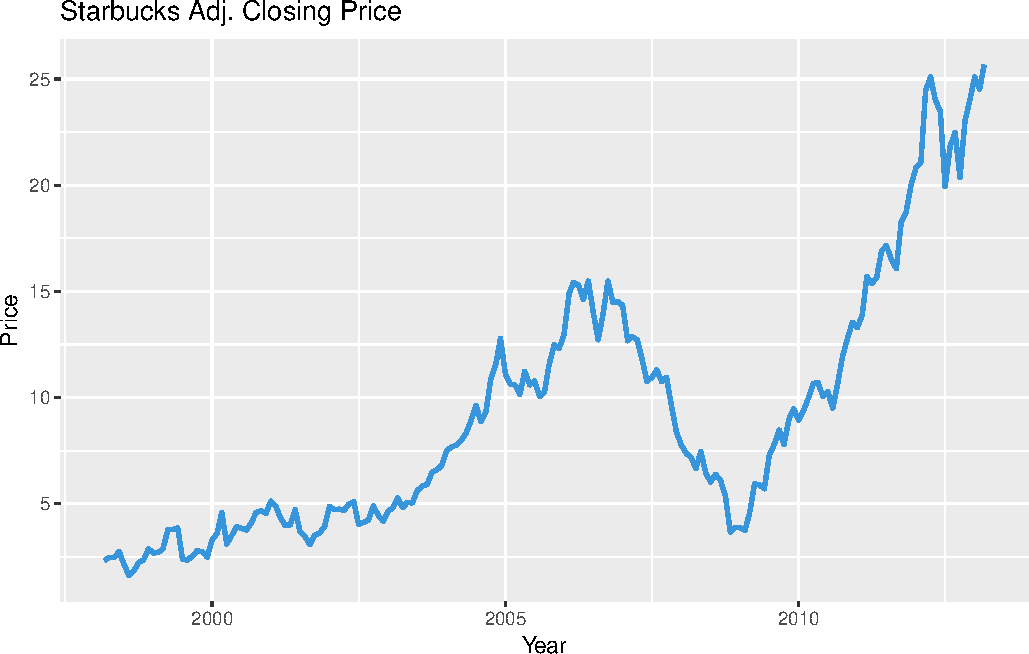
\includegraphics{homework_1_markdown_files/figure-latex/unnamed-chunk-13-1.pdf}

\paragraph{3) Compute monthly simple and continuously compounded
returns. Plot these returns separately first. Then also plot on the same
graph.}\label{compute-monthly-simple-and-continuously-compounded-returns.-plot-these-returns-separately-first.-then-also-plot-on-the-same-graph.}

\subparagraph{Computations}\label{computations}

\begin{Shaded}
\begin{Highlighting}[]
\NormalTok{starbucks[}\StringTok{'price_lag'}\NormalTok{] <-}\StringTok{ }\KeywordTok{lag}\NormalTok{(starbucks}\OperatorTok{$}\NormalTok{price)}
\NormalTok{starbucks[}\StringTok{'simple_return'}\NormalTok{] <-}\StringTok{ }\NormalTok{(starbucks}\OperatorTok{$}\NormalTok{price}\OperatorTok{-}\NormalTok{starbucks}\OperatorTok{$}\NormalTok{price_lag)}\OperatorTok{/}\NormalTok{(starbucks}\OperatorTok{$}\NormalTok{price_lag)}
\NormalTok{starbucks[}\StringTok{'cc_return'}\NormalTok{] <-}\StringTok{ }\KeywordTok{log}\NormalTok{(starbucks}\OperatorTok{$}\NormalTok{price) }\OperatorTok{-}\StringTok{ }\KeywordTok{log}\NormalTok{(starbucks}\OperatorTok{$}\NormalTok{price_lag)}
\end{Highlighting}
\end{Shaded}

\subparagraph{Simple Returns}\label{simple-returns}

\begin{Shaded}
\begin{Highlighting}[]
\KeywordTok{ggplot}\NormalTok{(}\DataTypeTok{data=}\NormalTok{starbucks, }\DataTypeTok{mapping=}\KeywordTok{aes}\NormalTok{(date, simple_return)) }\OperatorTok{+}
\StringTok{  }\KeywordTok{geom_line}\NormalTok{(}\DataTypeTok{color=}\StringTok{'black'}\NormalTok{, }\DataTypeTok{lwd=}\DecValTok{1}\NormalTok{) }\OperatorTok{+}
\StringTok{  }\KeywordTok{geom_hline}\NormalTok{(}\DataTypeTok{yintercept=}\DecValTok{0}\NormalTok{, }\DataTypeTok{linetype=}\StringTok{'dashed'}\NormalTok{) }\OperatorTok{+}
\StringTok{  }\KeywordTok{ylim}\NormalTok{(}\OperatorTok{-}\FloatTok{0.5}\NormalTok{, }\FloatTok{0.5}\NormalTok{) }\OperatorTok{+}
\StringTok{  }\KeywordTok{ggtitle}\NormalTok{(}\StringTok{'Starbucks Simple Returns'}\NormalTok{) }\OperatorTok{+}
\StringTok{  }\KeywordTok{xlab}\NormalTok{(}\StringTok{'Year'}\NormalTok{) }\OperatorTok{+}
\StringTok{  }\KeywordTok{ylab}\NormalTok{(}\StringTok{'Rate'}\NormalTok{)}
\end{Highlighting}
\end{Shaded}

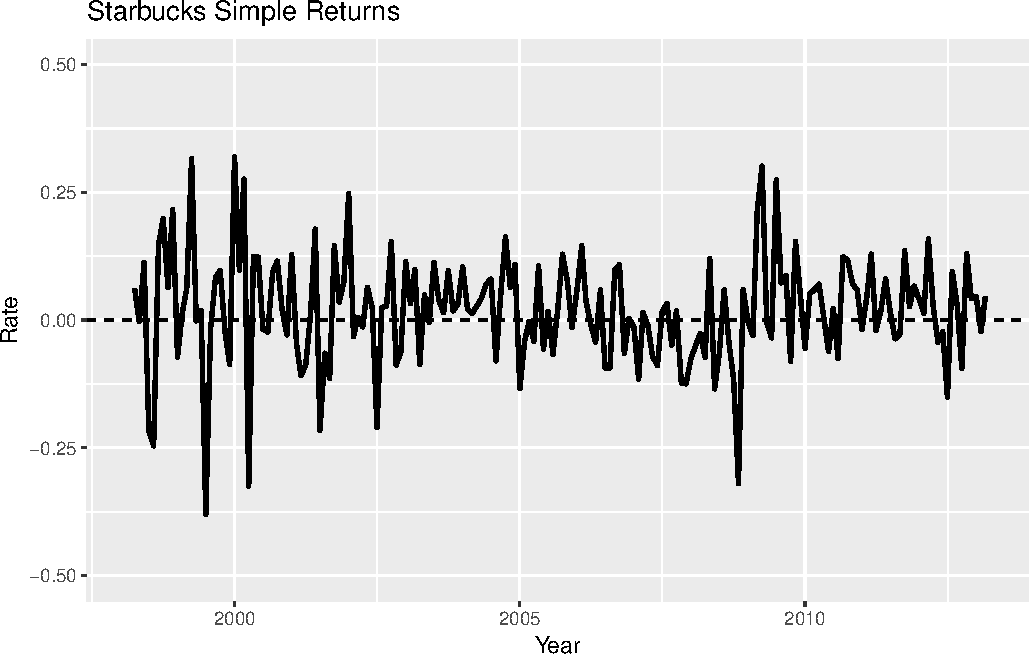
\includegraphics{homework_1_markdown_files/figure-latex/unnamed-chunk-15-1.pdf}

\subparagraph{CC Returns}\label{cc-returns}

\begin{Shaded}
\begin{Highlighting}[]
\KeywordTok{ggplot}\NormalTok{(}\DataTypeTok{data=}\NormalTok{starbucks, }\DataTypeTok{mapping=}\KeywordTok{aes}\NormalTok{(date, cc_return)) }\OperatorTok{+}
\StringTok{  }\KeywordTok{geom_line}\NormalTok{(}\DataTypeTok{color=}\StringTok{'green'}\NormalTok{, }\DataTypeTok{lwd=}\DecValTok{1}\NormalTok{) }\OperatorTok{+}
\StringTok{  }\KeywordTok{geom_hline}\NormalTok{(}\DataTypeTok{yintercept=}\DecValTok{0}\NormalTok{, }\DataTypeTok{linetype=}\StringTok{'dashed'}\NormalTok{) }\OperatorTok{+}
\StringTok{  }\KeywordTok{ylim}\NormalTok{(}\OperatorTok{-}\FloatTok{0.5}\NormalTok{, }\FloatTok{0.5}\NormalTok{) }\OperatorTok{+}
\StringTok{  }\KeywordTok{ggtitle}\NormalTok{(}\StringTok{'Starbucks CC Returns'}\NormalTok{) }\OperatorTok{+}
\StringTok{  }\KeywordTok{xlab}\NormalTok{(}\StringTok{'Year'}\NormalTok{) }\OperatorTok{+}
\StringTok{  }\KeywordTok{ylab}\NormalTok{(}\StringTok{'Rate'}\NormalTok{)}
\end{Highlighting}
\end{Shaded}

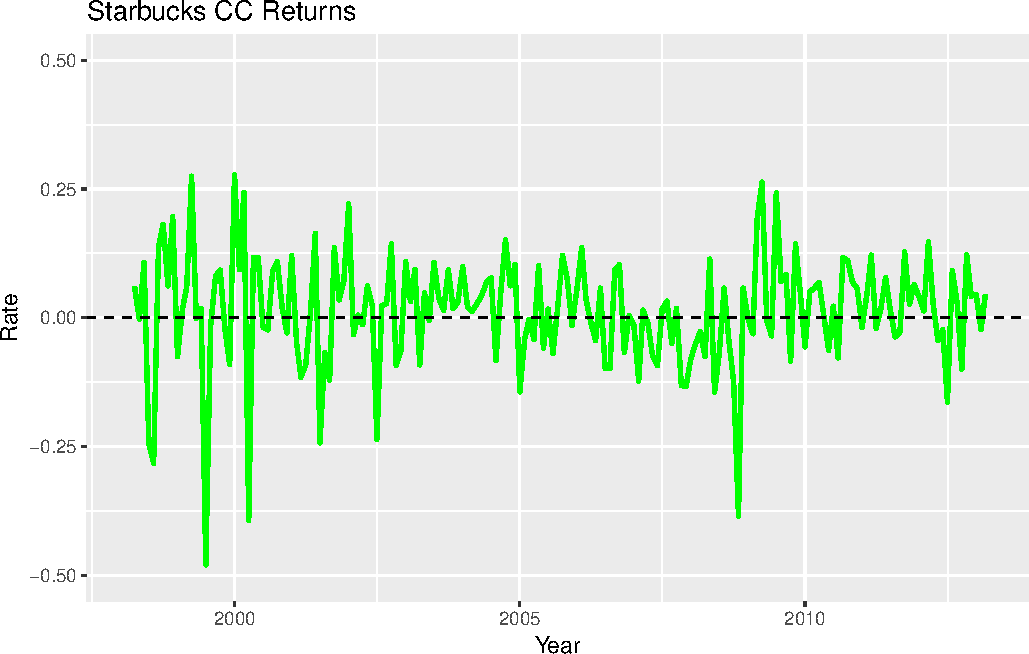
\includegraphics{homework_1_markdown_files/figure-latex/unnamed-chunk-16-1.pdf}

\subparagraph{Simple and CC Returns}\label{simple-and-cc-returns}

\begin{Shaded}
\begin{Highlighting}[]
\CommentTok{# Rearrange dataframe for multiple series plotting}
\NormalTok{ss <-}\StringTok{ }\NormalTok{starbucks[, }\KeywordTok{c}\NormalTok{(}\DecValTok{1}\NormalTok{, }\DecValTok{4}\NormalTok{, }\DecValTok{5}\NormalTok{)]}
\NormalTok{dd =}\StringTok{ }\KeywordTok{melt}\NormalTok{(ss, }\DataTypeTok{id=}\KeywordTok{c}\NormalTok{(}\StringTok{"date"}\NormalTok{))}

\KeywordTok{ggplot}\NormalTok{(}\DataTypeTok{data=}\NormalTok{starbucks) }\OperatorTok{+}
\StringTok{  }\KeywordTok{geom_line}\NormalTok{(}\DataTypeTok{mapping=}\KeywordTok{aes}\NormalTok{(date, simple_return), }\DataTypeTok{color=}\StringTok{'black'}\NormalTok{, }\DataTypeTok{lwd=}\FloatTok{0.5}\NormalTok{) }\OperatorTok{+}
\StringTok{  }\KeywordTok{geom_line}\NormalTok{(}\DataTypeTok{mapping=}\KeywordTok{aes}\NormalTok{(date, cc_return), }\DataTypeTok{color=}\StringTok{'green'}\NormalTok{, }\DataTypeTok{lwd=}\FloatTok{0.5}\NormalTok{) }\OperatorTok{+}
\StringTok{  }\KeywordTok{geom_hline}\NormalTok{(}\DataTypeTok{yintercept=}\DecValTok{0}\NormalTok{, }\DataTypeTok{linetype=}\StringTok{'dashed'}\NormalTok{) }\OperatorTok{+}
\StringTok{  }\KeywordTok{ylim}\NormalTok{(}\OperatorTok{-}\FloatTok{0.5}\NormalTok{, }\FloatTok{0.5}\NormalTok{) }\OperatorTok{+}
\StringTok{  }\KeywordTok{ggtitle}\NormalTok{(}\StringTok{'Starbucks Simple and CC Returns'}\NormalTok{) }\OperatorTok{+}
\StringTok{  }\KeywordTok{xlab}\NormalTok{(}\StringTok{'Year'}\NormalTok{) }\OperatorTok{+}
\StringTok{  }\KeywordTok{ylab}\NormalTok{(}\StringTok{'Rate'}\NormalTok{)}
\end{Highlighting}
\end{Shaded}

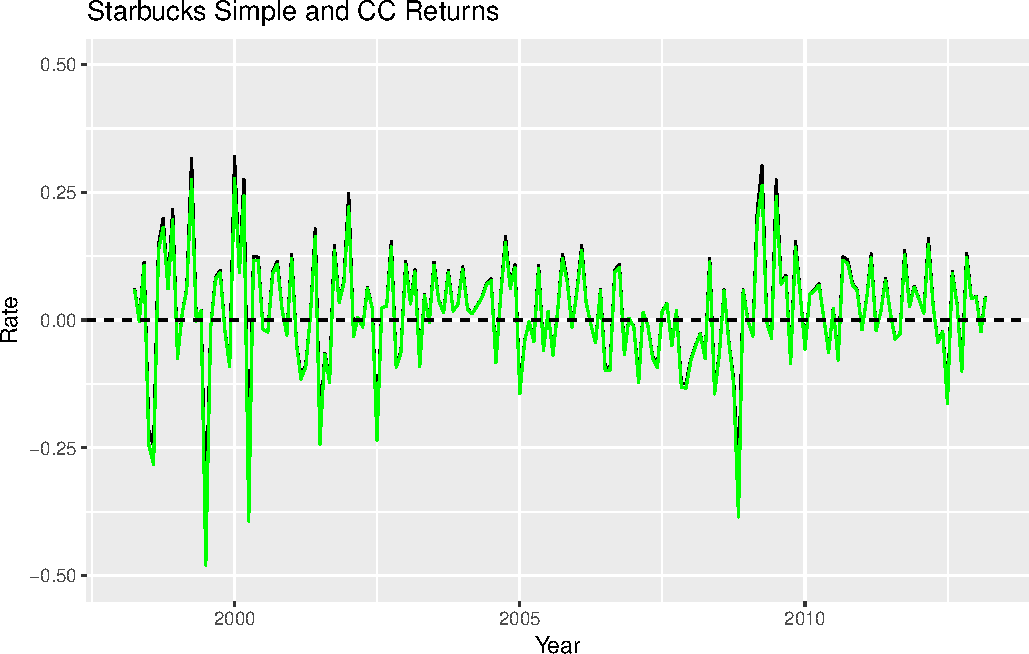
\includegraphics{homework_1_markdown_files/figure-latex/unnamed-chunk-17-1.pdf}


\end{document}
